\section{SQL и NoSQL. Определения. Сравнения. Сценарии использования.}

\D{
    База данных - это набор сведений об объектах, структурированный 
    определенным образом.
}

\subsection*{SQL}

\D{
    SQL - набор структурированных таблиц. Каждая строка - объект данных, столбец
    - информационное поле.

    Реляционные базы данных строятся с использованием языка
    структурированных запросов (SQL) для
    создания, хранения, обновления и извлечения данных.
}

Данные организуются в таблицах.

Каждый столбец содержит определенную атрибутивную информацию, а
свойства столбца определяют тип данных (например, числовые или текстовые
данные) и диапазон, который он может принимать.

Каждая таблица имеет первичный ключ для уникальной идентификации сущности.

Поскольку стандартным языком программирования является SQL, реляционные базы данных
используют DDL для изменения схемы в режиме реального времени .

Это позволяет пользователям баз данных добавлять новые таблицы и столбцы,
переименовывать отношения и вносить различные другие изменения в режиме реального времени без
остановки операций с базой данных.

Избыточность уменьшается путем нормализации.

Из-за популярности довольно просто обслуживать.


\subsection*{NoSQL}

\D{
    NoSQL - являются нетабличными базами данных
    и хранят данные иначе, чем реляционные таблицы. Базы данных
    NoSQL бывают разных типов в зависимости от модели данных.

    Основными типами являются документ, ключ -значение, широкий
    столбец и граф.
}

Не использует SQL. Структура не регламентирована.

\begin{figure}[ht]
	\centering
	\begin{minipage}[b]{0.65\textwidth}
		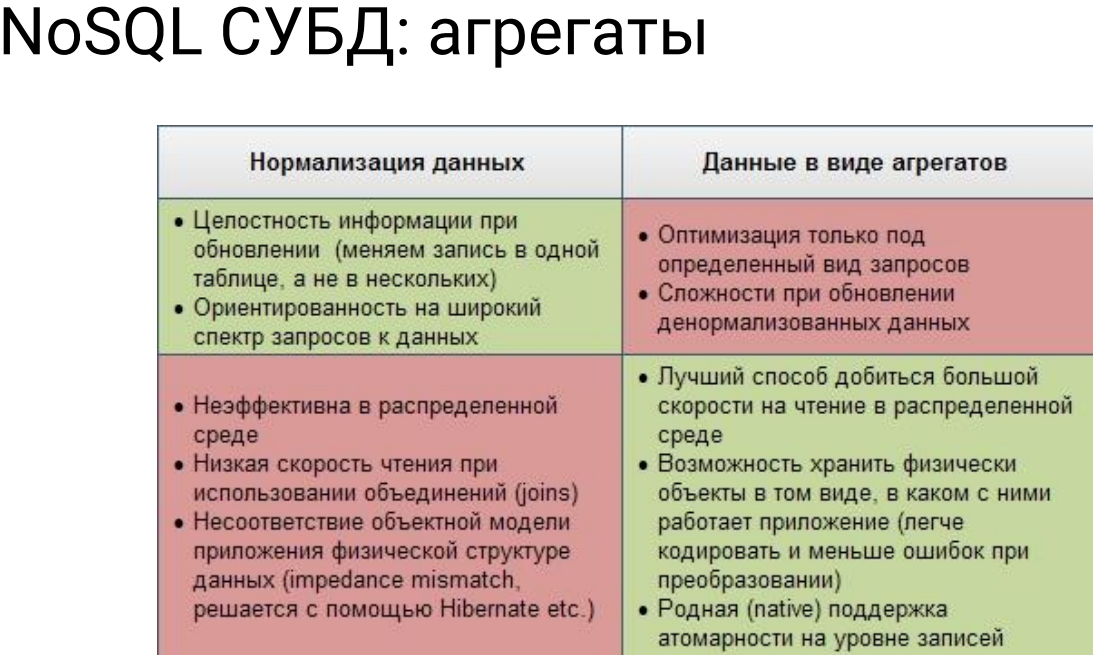
\includegraphics[width=\textwidth]{images/agg.png}
        \caption{Агрегаты}
	\end{minipage}
\end{figure}

\D{
    ACID - требования к транзакционной системе.
    \begin{itemize}
        \item Атомарность - ни одна транзакция не будет частично зафиксирована.
        \item Согласованность - любая операция приводит только к правильному результату.
        \item Изоляция - параллельные операции не влияют на результат текущей.
        \item Долговечность - в случае сбоя системы результат успешной
        операции должен сохраняться после восстановления.
    \end{itemize}
}

Хотим все делать быстрее, но ускорять железки (вертикально
масштабировать) - дорого. Масштабируем горизонтально =
делаем несколько серверов.

\D{
    Репликация - копирование данных на другие узлы при
    обновлении. Позволяет как добиться большей масштабируемости,
    так и повысить доступность и сохранность данных. Принято
    подразделять на два вида.
    \begin{itemize}
        \item Master-Slave
        \item Peer-to-Peer
    \end{itemize}

    Шардинг - каждый узел отвечает за часть набора данных.
}

\subsection*{VS}

Za SQL:
\begin{itemize}
    \item Прост в применении
    \item ACID
    \item Структура лучше
    \item Трудоемкий дизайн
    \item Вертикальное масштабирование
    \item Фиксированная схема
\end{itemize}

Za NoSQL:
\begin{itemize}
    \item Быстрое развитие
    \item Принцип BASE
    \item Работает быстрее
    \item Нет инвестиций в дизайн
    \item Горизонтальное масштабирование
    \item Динамическая схема
\end{itemize}
